% EMPD chapter

\chapter{The EMPD and POLNET web-interfaces}

\label{chp:empd}

\begin{refsection}

\section{Summary}\label{sec:empd-summary}

\begin{figure}
	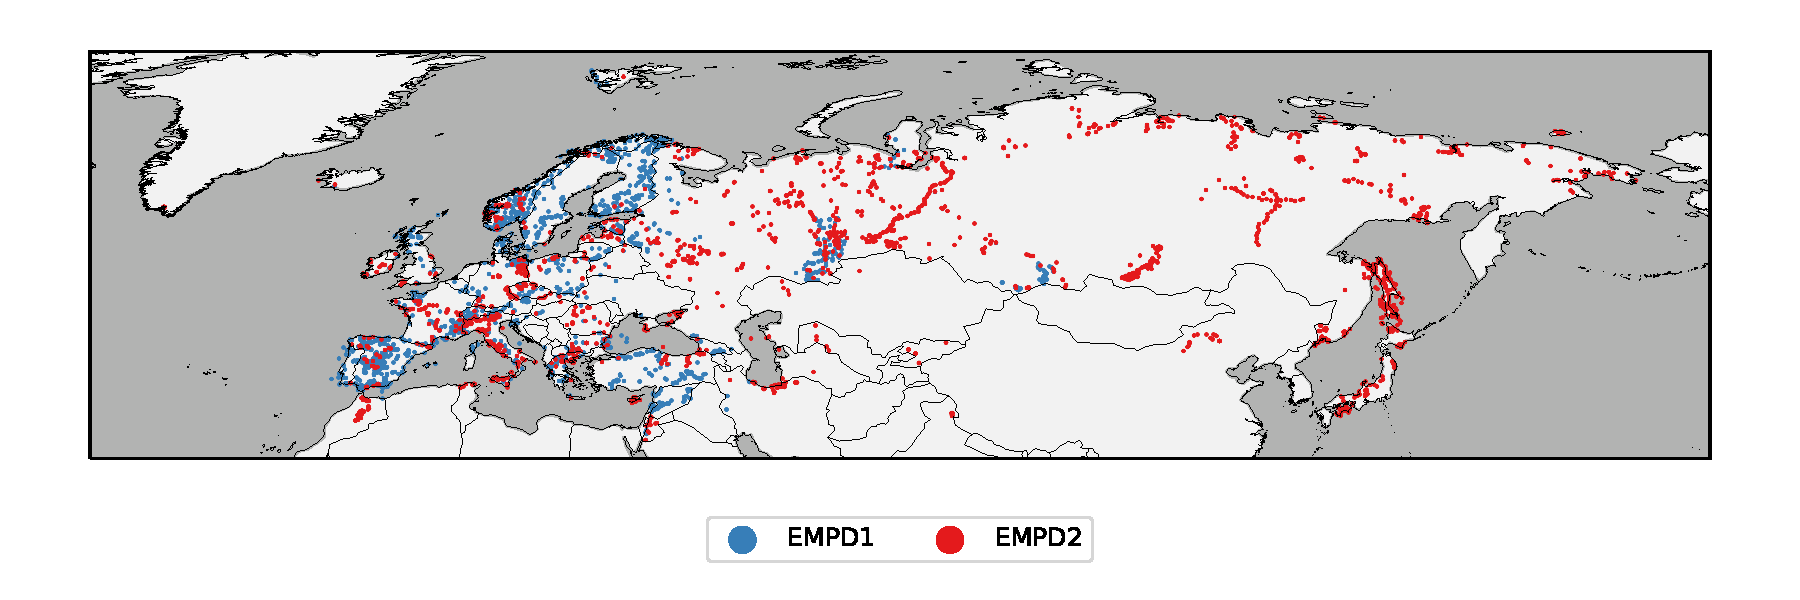
\includegraphics[width=\linewidth]{empd-figures/empd-sites.pdf}
	\caption[Modern calibration samples in the EMPD]{Modern calibration samples in the \gls{empd}.\todo[inline]{needs to be formatted (see printed version)}}
	\label{fig:empd-sites}
\end{figure}

The \glslink{empd}{Eurasian (née European) Modern Pollen Database (EMPD)} was established in 2013 as a public database of quality controlled and standardized modern pollen surface sample data to compliment the European Pollen Database (EPD) for fossil pollen \citep{DavisZanonCollinsEtAl2013}. The first version of the \gls{empd} (referenced herein as the \gls{empd}1) contained almost 5000 samples, submitted by over 40 individuals and research groups from all over Europe. Over the last 6 years more data has continued to be submitted, and more efforts have been made to incorporate more data held in open data repositories such as PANGAEA, and as supplementary information in published studies. This data is now released as the Eurasian Modern Pollen Database, version 2 \citep{DavisChevalierSommerEtAlinprep} with an increase of 80 percent to 8663 samples (see figure \ref{fig:empd-sites}).

The \gls{empd} remains the only public and open access database of modern pollen samples covering the Eurasian continent and is entirely driven by the community of its data contributors. This effort of creating an open and accessible database led to the development of new open source data management tools that we present in this chapter. The \gls{empd}2 is now hosted on the version control platform Github, with a dedicated web viewer at \href{https://EMPD2.github.io}{EMPD2.github.io} and an automated administration app, the \gls{empd}-admin (see table \ref{tab:empd-links} for a list of the web resources). The new web-viewer provides an intuitive interface into the database and displays the essential meta information for every sample, as well as the pollen and climate data in a comprehensive bar plot. The integration with the \gls{empd}-admin provides a simplified and transparent administration of multiple contributions from different sources and people to the database. All web components are hosted without any additional costs. The integration for the \gls{empd}, that we present here, is only one example of a regional database. This framework can be extended to make other community-based (regional) pollen databases accessible, for instance the \glsfirst{lapd} \citep{FlantuaHooghiemstraGrimmEtAl2015} or \glsfirst{apd} \citep{VincensLezineBuchetEtAl2007}. Especially the light-weight \gls{empd}-viewer web interface can be ported to other database (as shown in section \ref{sec:polnet-viewer}) to make heterogeneous data accessible to the broad public.

\begin{table}
	\caption{EMPD Web resources}
	\label{tab:empd-links}
	\begin{tabular}{|l|p{0.25\linewidth}|c|}
		\hline 
		& Description & Online Access \\ 
		\hline
		EMPD2 & Github Organization & \href{https://github.com/EMPD2}{github.com/EMPD2} \\
		\hline 
		\multirow{3}{*}{EMPD-Viewer} & \multirow{3}{\linewidth}{Map-based web interface to the EMPD database} & \href{https://github.com/EMPD2/EMPD-viewer}{github.com/EMPD2/EMPD-Viewer} \\
		& & \href{https://empd2.github.io/}{empd2.github.io} \\
		& & \\
		\hline 
		\multirow{3}{*}{EMPD-Data} & \multirow{3}{\linewidth}{Version controlled data repository of the EMPD} & \href{https://github.com/EMPD2/EMPD-data}{github.com/EMPD2/EMPD-data}  \\ 
		& & \\
		& & \\
		\hline 
		\multirow{3}{*}{EMPD-Admin} &  \multirow{3}{\linewidth}{Automated administration web app for the EMPD} & \href{https://github.com/EMPD2/EMPD-admin}{github.com/EMPD2/EMPD-admin} \\ 
		& & \href{https://empd-admin.herokuapp.com/}{empd-admin.herokuapp.com} \\ 
		& & \href{https://EMPD2.github.io/EMPD-admin}{EMPD2.github.io/EMPD-admin} \\ 
		\hline 
	\end{tabular} 
\end{table}

\section{The EMPD web framework}\label{sec:empd-web-framework}

The EMPD web framework is built on very common open source software development tools that have been adopted for a transparent data management, in favor of open science. The \gls{empd} is now hosted on the web platform Github at \href{https://github.com/EMPD2}{github.com/EMPD2}. This web platform, free of charge, hosts the source code for many popular open source software packages but can also be used to host a diverse, but small database (in terms of megabytes), such as the \gls{empd}. Github builts upon the version control system \textit{git} that transparently manages changes to documents by providing a full history of their revisions. The web platform is intrinsically designed for community-based projects that focus on collaboration and contains many features for a transparent communication between users, maintainers and contributors of a project. Besides others, the platform provides repository (i.e. project) specific discussion pages, so-called issues, where users can provide feedback, report bugs, or discuss any other aspect of the project. These issues are often linked to so-called pull requests, where each pull request is a proposal for a change in the source files of the project. This is then discussed between project maintainer and contributor in a dedicated discussion/review page.

Another common feature for Github repositories are integrations with so-called \glsfirst{ci} services, e.g. for automated testing and/or packaging the software. These services run predefined scripts (for example test scripts) every time someone contributes to the repository, or creates a pull request.

The following sections describe how these software development tools are implemented in the three components of the \gls{empd} web framework, the \gls{empd}-viewer (section \ref{sec:empd-viewer}), the \gls{empd} data repository (section \ref{sec:empd-data}) and the \gls{empd}-admin (section \ref{sec:empd-admin}).

\subsection{The EMPD viewer}\label{sec:empd-viewer}

\begin{figure}[h]
	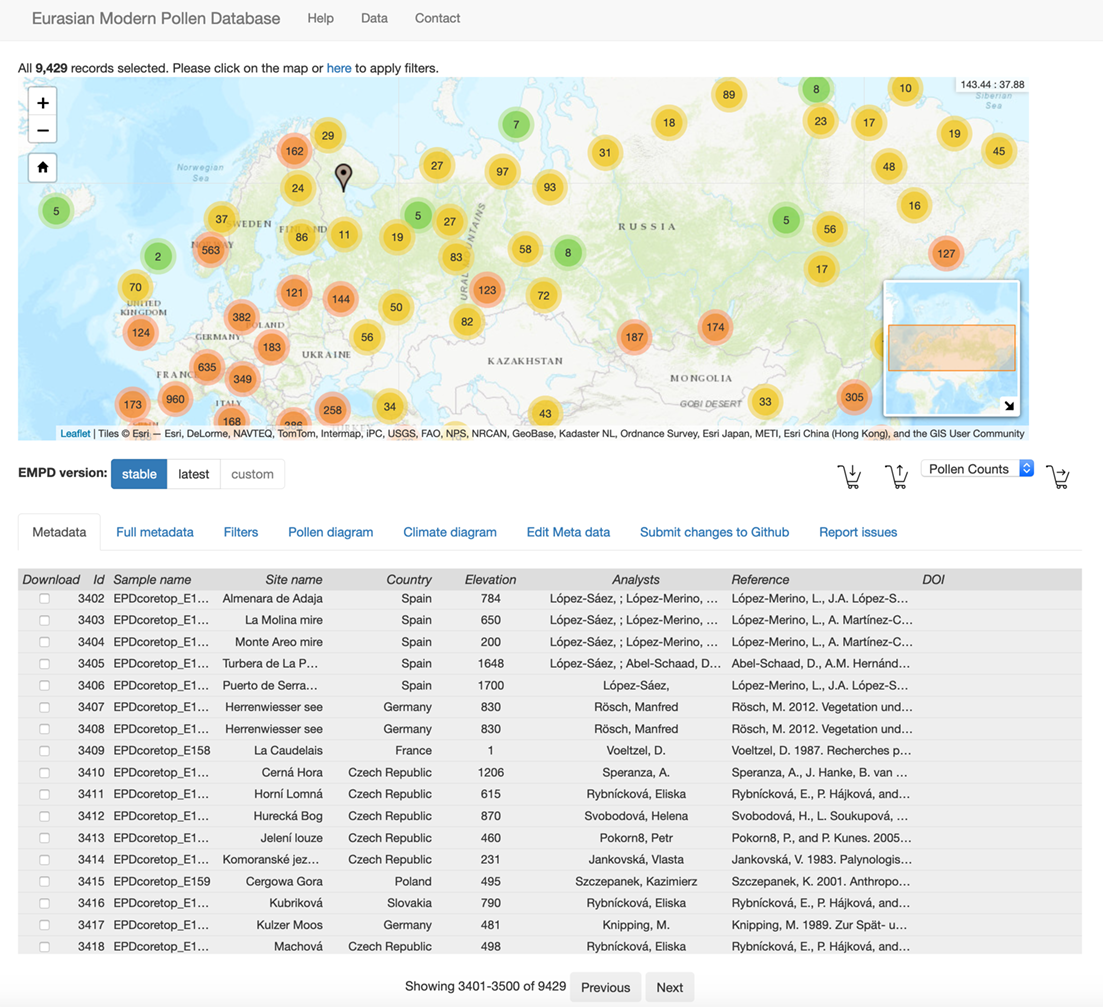
\includegraphics[width=\linewidth]{empd-figures/screenshot-compr.png}
	\caption{Screenshot of the EMPD viewer}
	\label{fig:empd-viewer}
\end{figure}

The main public interface into the \gls{empd} is an interactive web viewer accessible
from \href{https://EMPD2.github.io}{EMPD2.github.io}. This JavaScript-based application (see figure \ref{fig:empd-viewer} for a screenshot) provides an intuitive interface into the database without requiring any particular computer expertise. It enables the user to view the data on a map and to select and download subsets of the database. The webpage involves no server-side processing and such it can be hosted for free using the service provided by Github Pages (\href{https://pages.github.com/}{pages.github.com}). This provides a stable access to the database, independent of funding availabilities.

\subsubsection{The Web Interface}

The EMPD-Viewer has been initially based on the climate proxies finder \citep{BollietBrockmannMassonDelmotteEtAl2016, Brockmann2016} which can still be seen in it the layout and design of its graphical interface (i.e. its front-end). The code base, however, has been changed entirely, updated to the latest available versions of the underlying JavaScript dependencies and extended with multiple additional tools, shown in table \ref{tab:empd-viewer-tools}. The central element of the viewer is a map to show the sample locations. It also allows to intuitive access to the essential meta data of every sample through the popup of the corresponding marker on the map. The detailed meta data can also be seen in the meta data table, together with all the other samples. Another key element of the viewer are the meta data filters, that subset the data using efficient and intuitive filtering tools. This allows to search the database\todo{needs implementation}, or to select specific countries, climatic regimes, sample types, samples of a specific data contributor/analyst, and more.

Additional information on the sample is revealed through a bar diagram of the associated pollen data, which is dynamically created when the user clicks on the sample. The viewer also displays monthly, seasonal and annual precipitation and temperature values at the side, based on the WorldClim dataset, version 2 \citep{FickHijmans2017}.

Finally, the viewer contains elements that allow scientists to contribute to the database, even without dedicated knowledge about the Github framework. The meta data editor allows to edit a sample and then submit it via the data submission form. The request is handled by the \gls{empd}-admin webapp (see section \ref{sec:empd-admin}) that pushes the data to the corresponding pull request on Github that is then reviewed by the core database maintainers. Another implemented element is an issue report form that allows the user to highlight erroneous sample information which is then, again through the \gls{empd}-admin, submitted as a Github issue to the data repository.

The web app is fully integrated into the Github framework of the \gls{empd} and loads the displayed data from the online repository. As such, it also provides a further quality control check and allows the data contributors/maintainers to review and edit new contributions before they are merged into the database.

\afterpage{
	\begin{longtable}{c}
		\caption[Tools in the EMPD viewer]{Tools in the \gls{empd} viewer} \label{tab:empd-viewer-tools} \\
		\endfirsthead
		\caption{Tools in the EMPD viewer (continued)}
		\endhead
		\hline
		\tabularnewline
		Map interface \\
		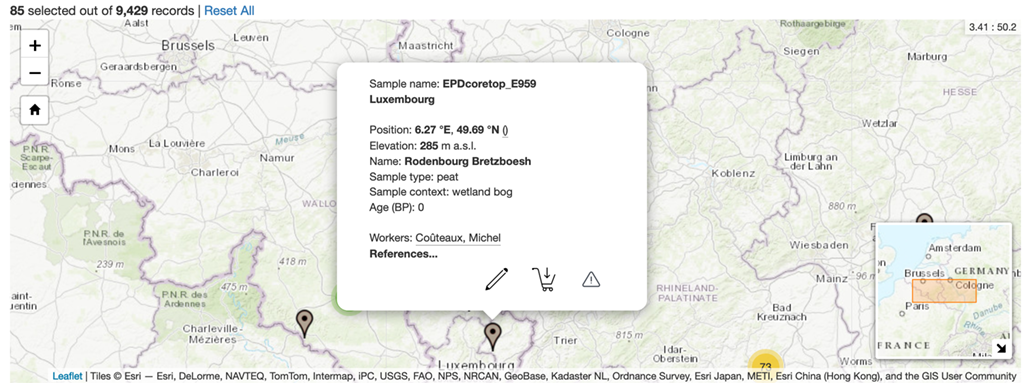
\includegraphics[width=\linewidth]{empd-figures/map-compr.png} \\
		\todo[inline]{may need a higher resolution} \\
		\hline\hline
		\tabularnewline
		Meta data table \\
		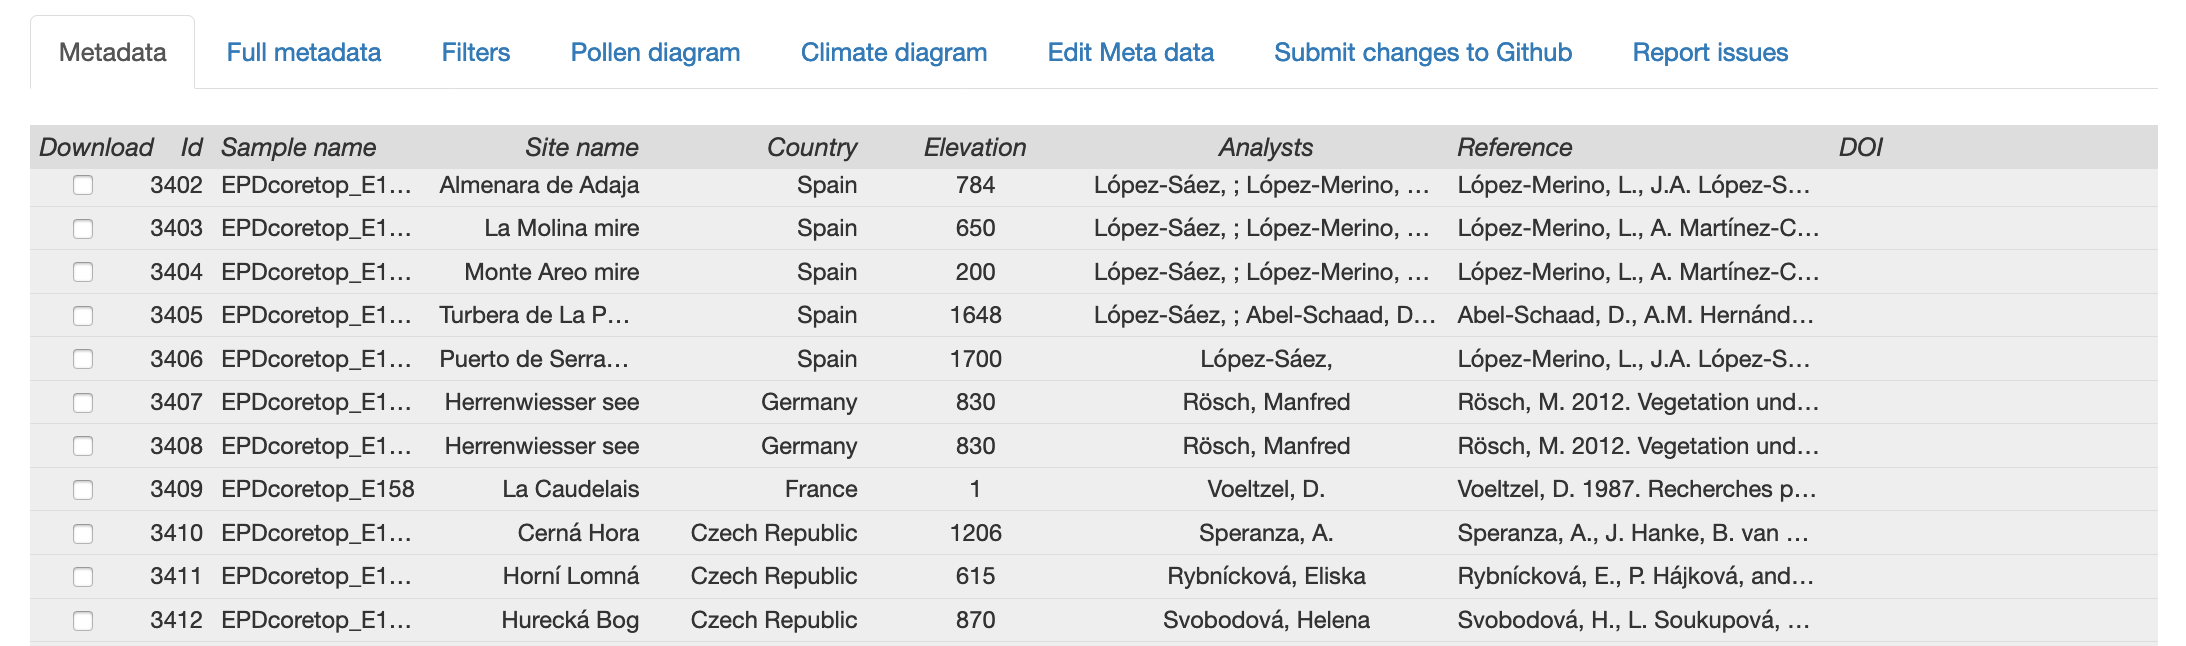
\includegraphics[width=\linewidth]{empd-figures/meta-data-table.png} \\
		\hline\hline
		\tabularnewline
		Pollen Data \\
		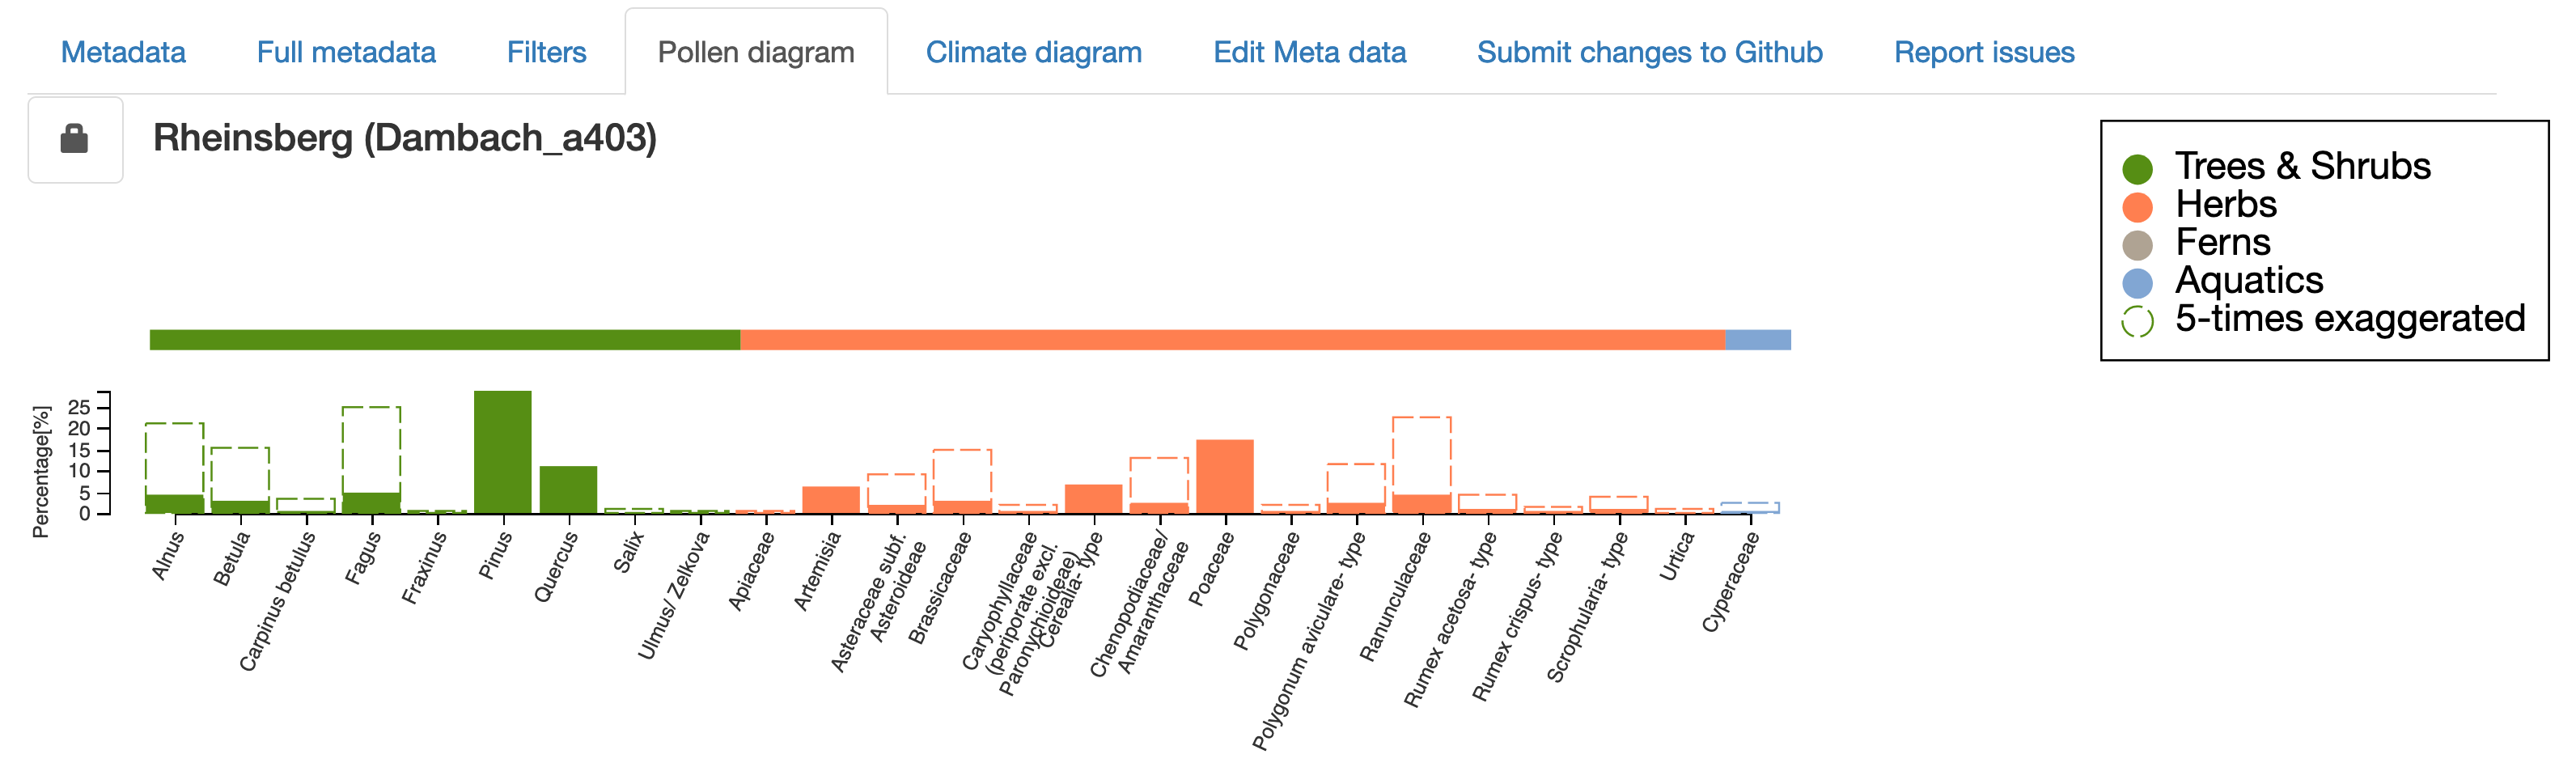
\includegraphics[width=\linewidth]{empd-figures/pollen-bar-diagram.png} \\
		\hline\hline
		\tabularnewline
		Climate Data \\
		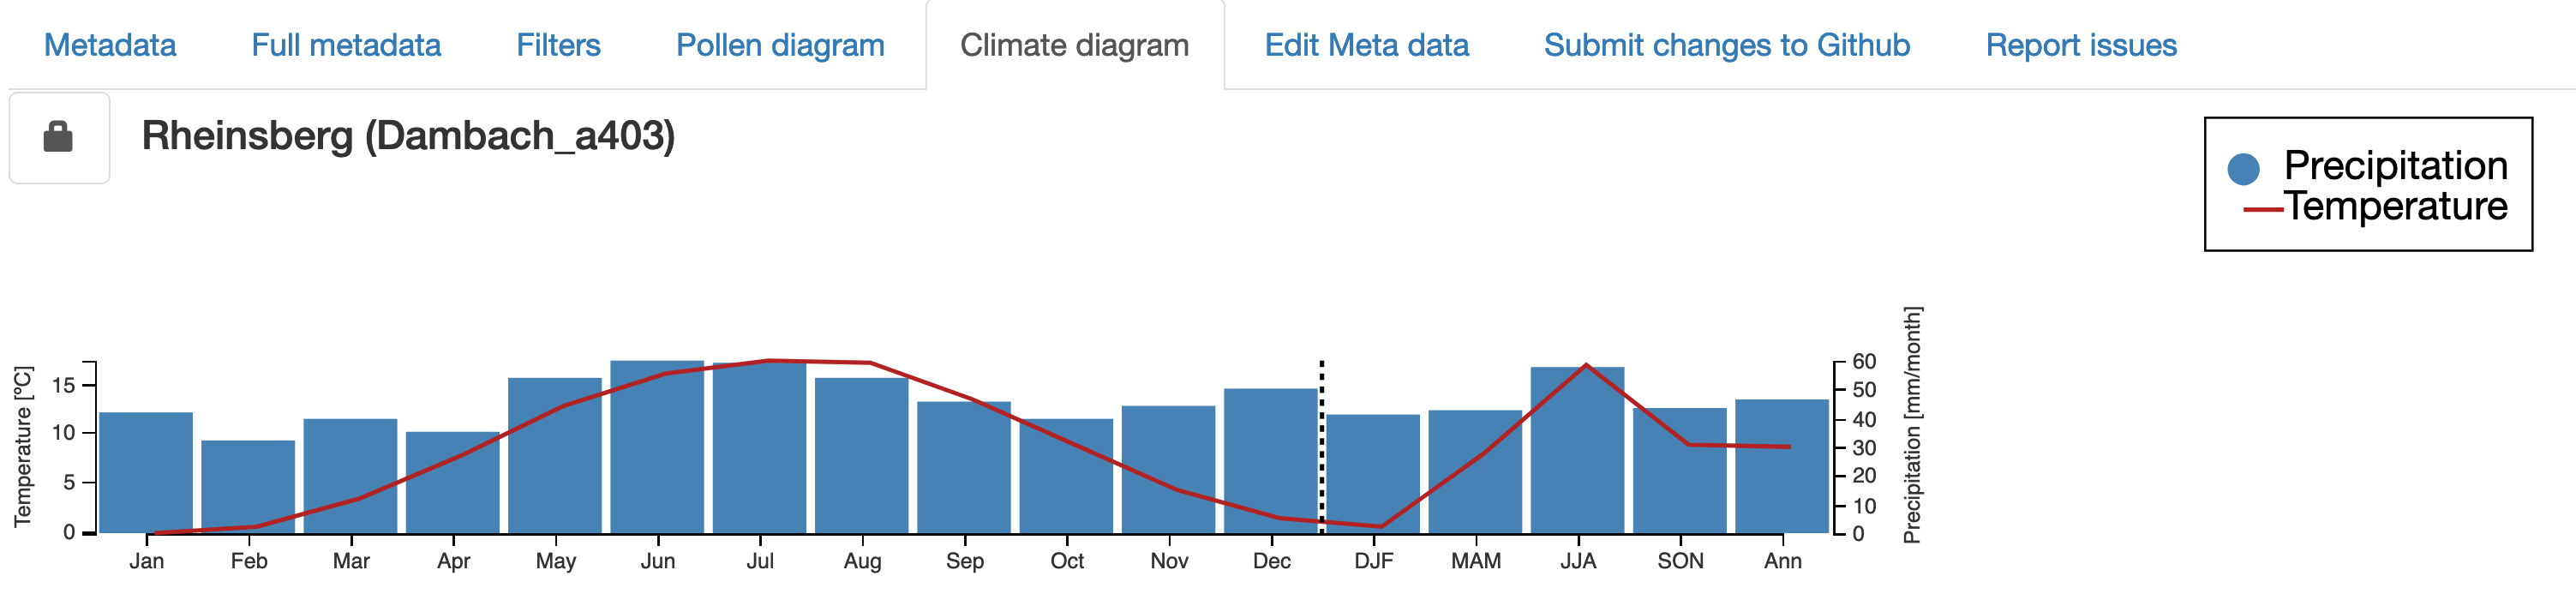
\includegraphics[width=\linewidth]{empd-figures/climate-diagram.png} \\
		\newpage \\
		\hline
		\tabularnewline
		Meta data filter \\
		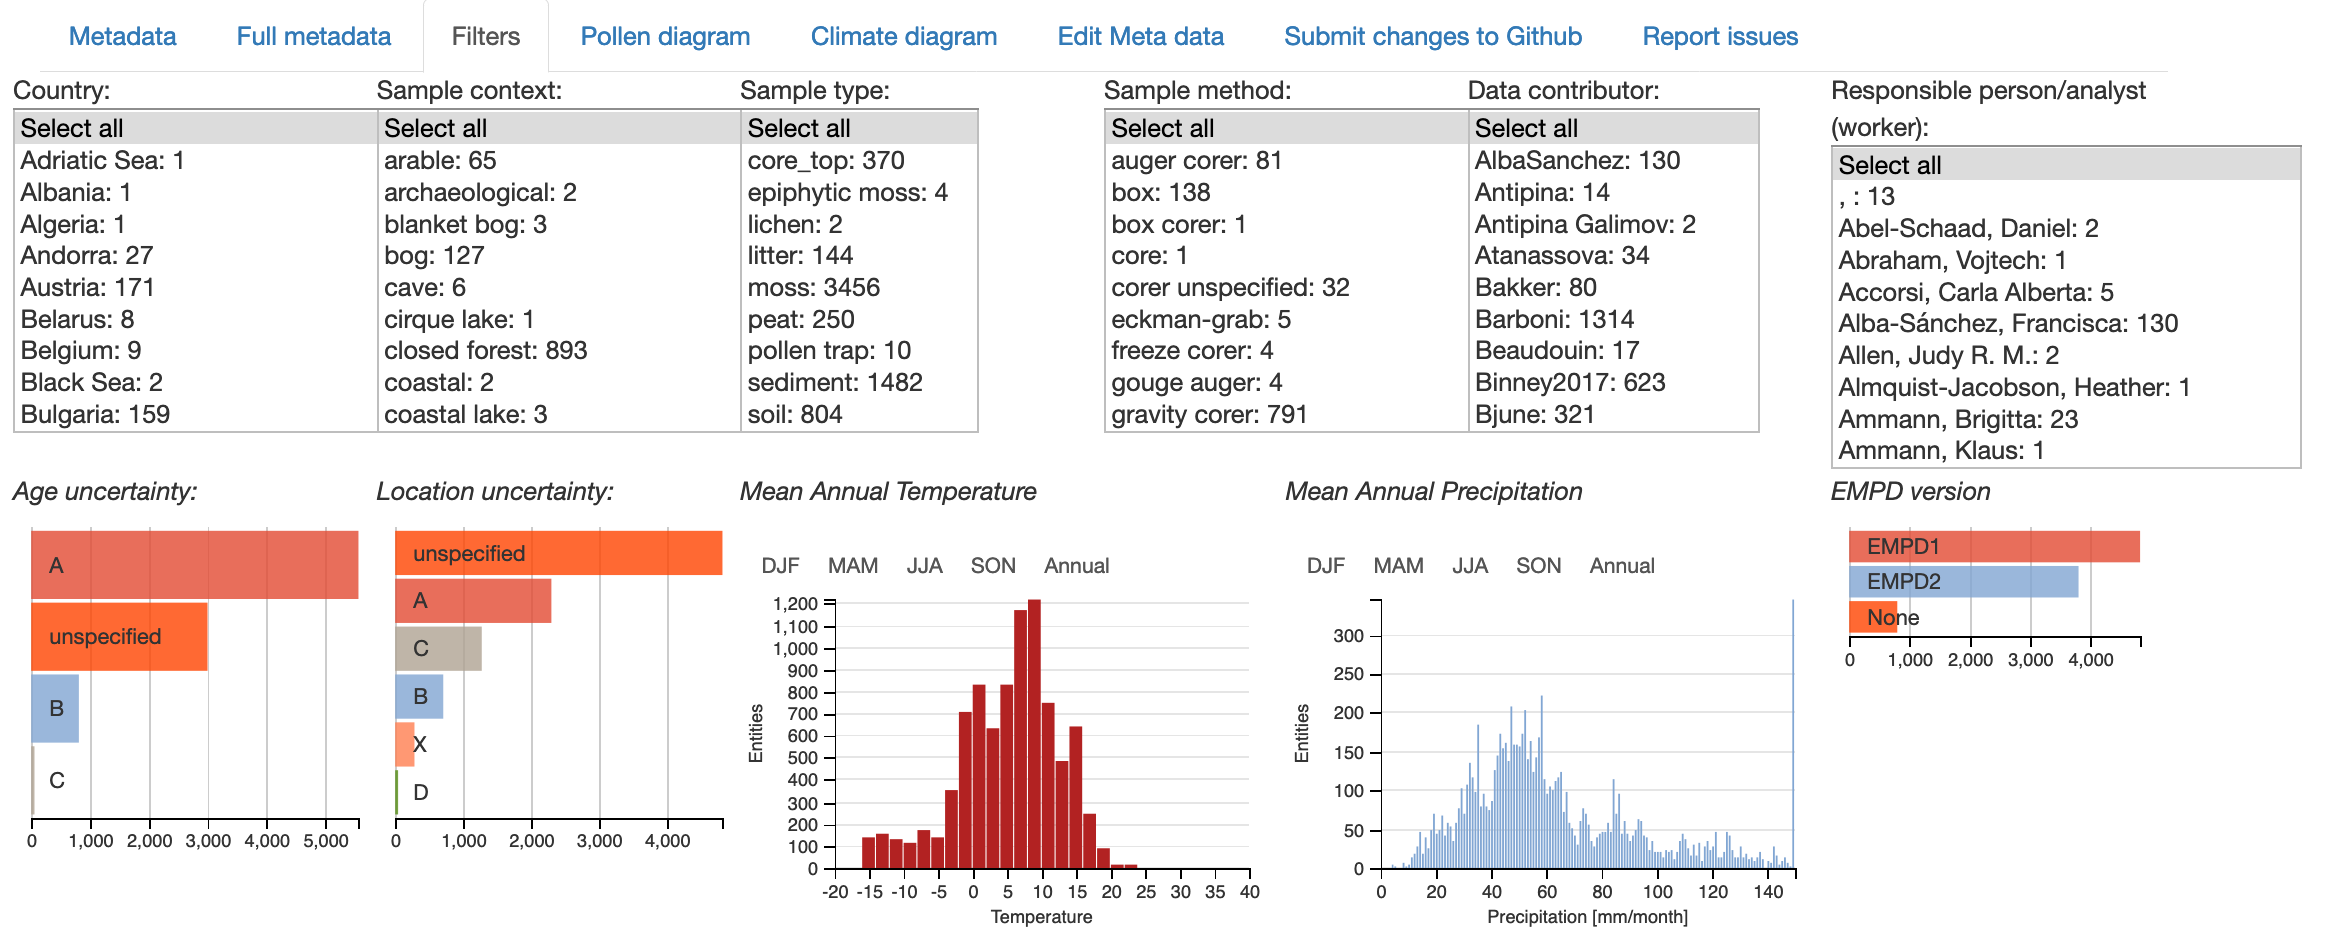
\includegraphics[width=\linewidth]{empd-figures/filter.png} \\
		\hline
		\tabularnewline
		Meta Data Editor \\
		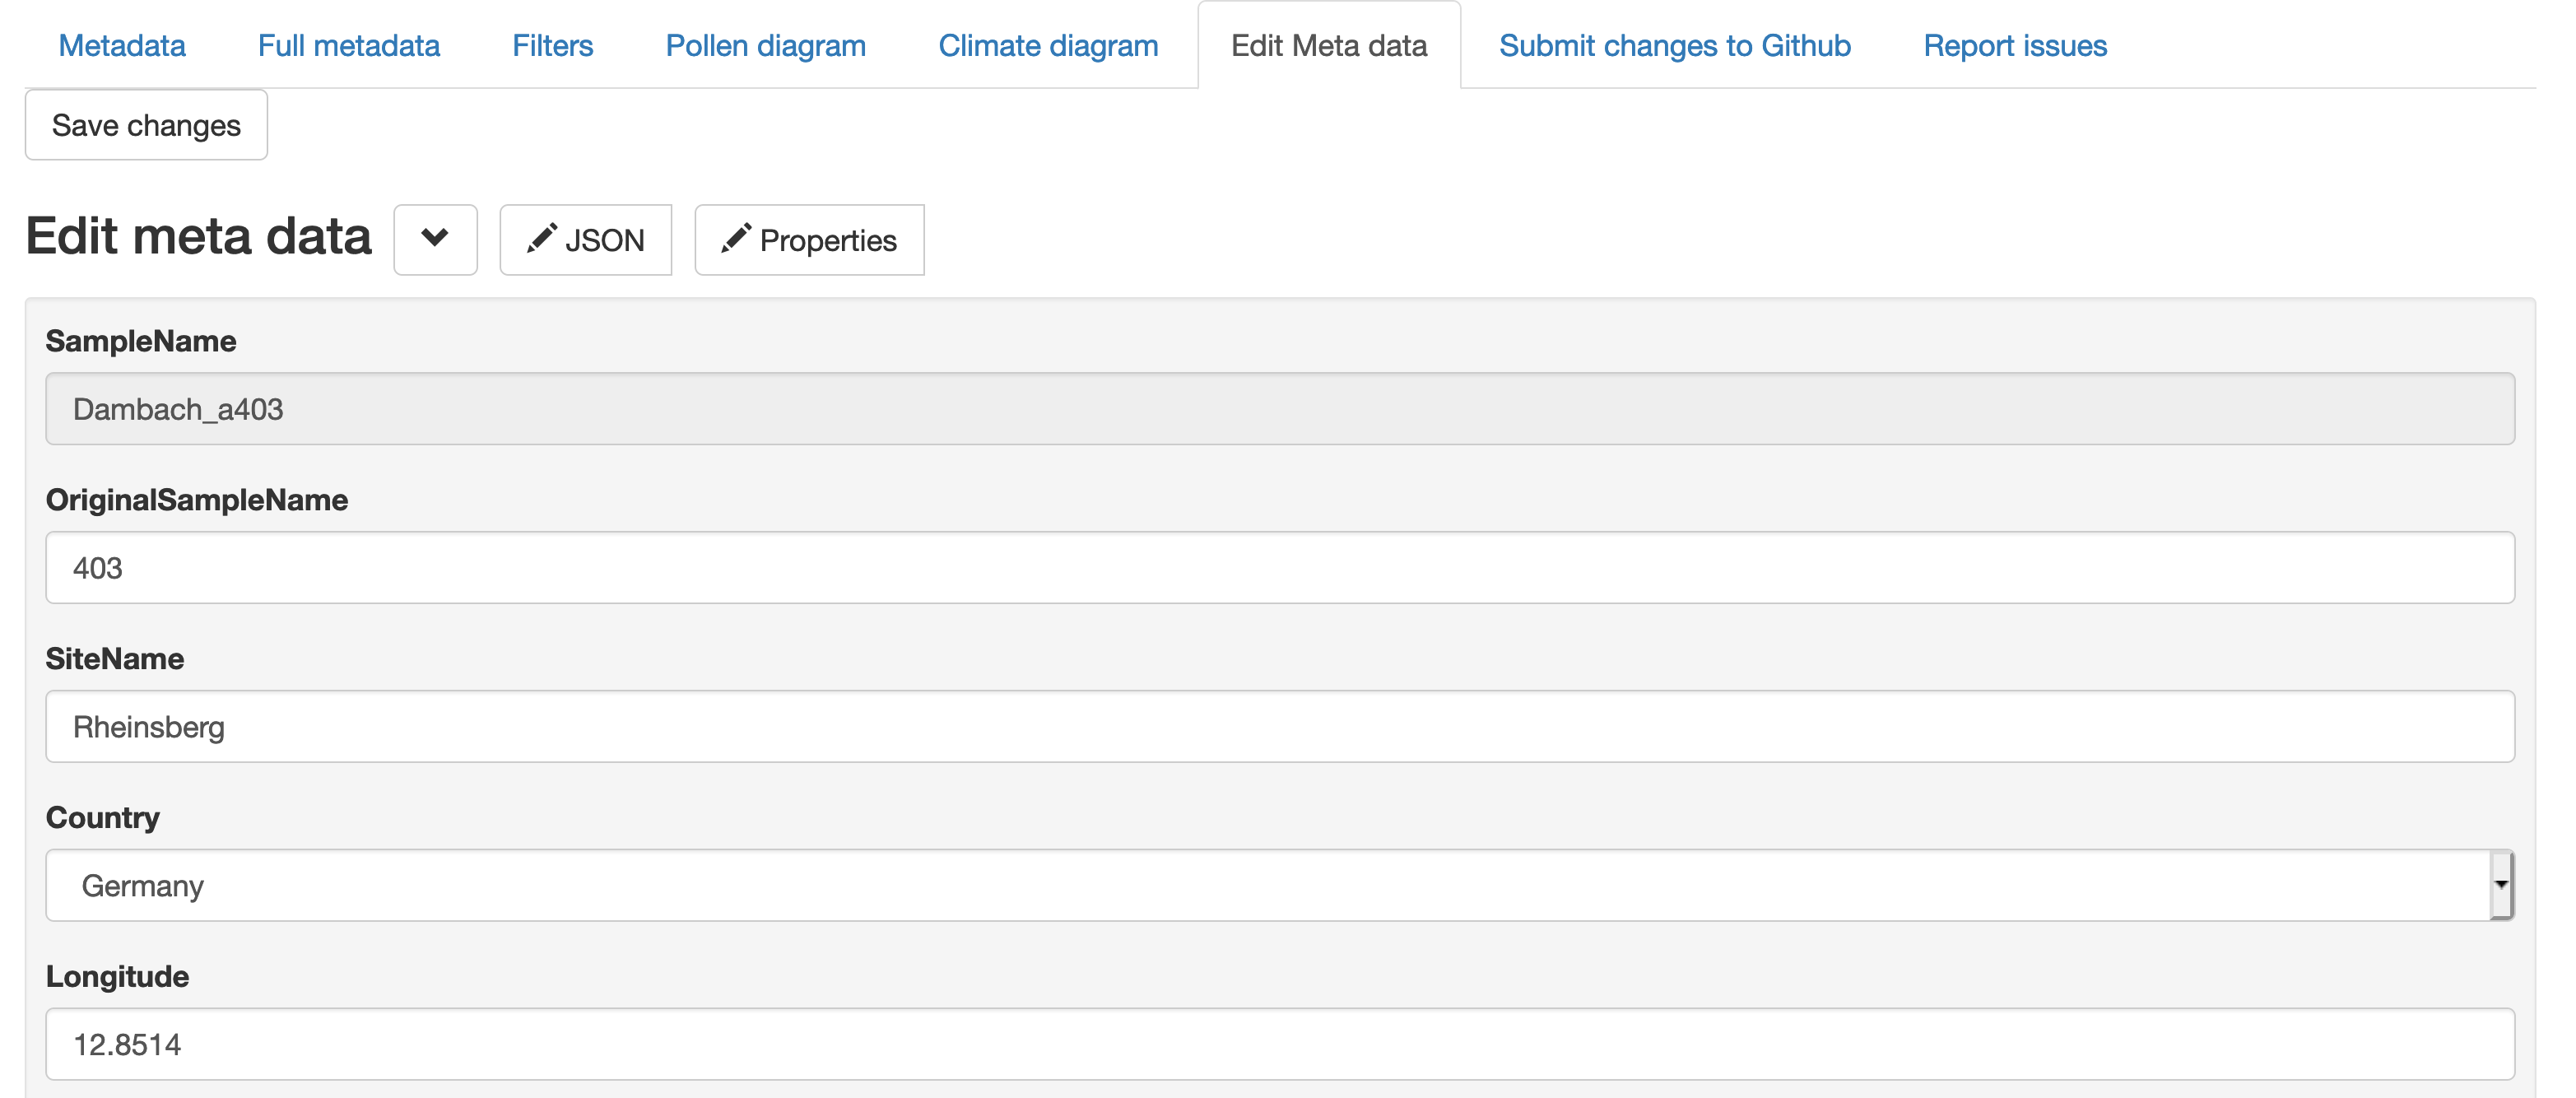
\includegraphics[width=\linewidth]{empd-figures/meta-data-editor.png} \\
		\hline
		\tabularnewline
		Issue submission form \\
		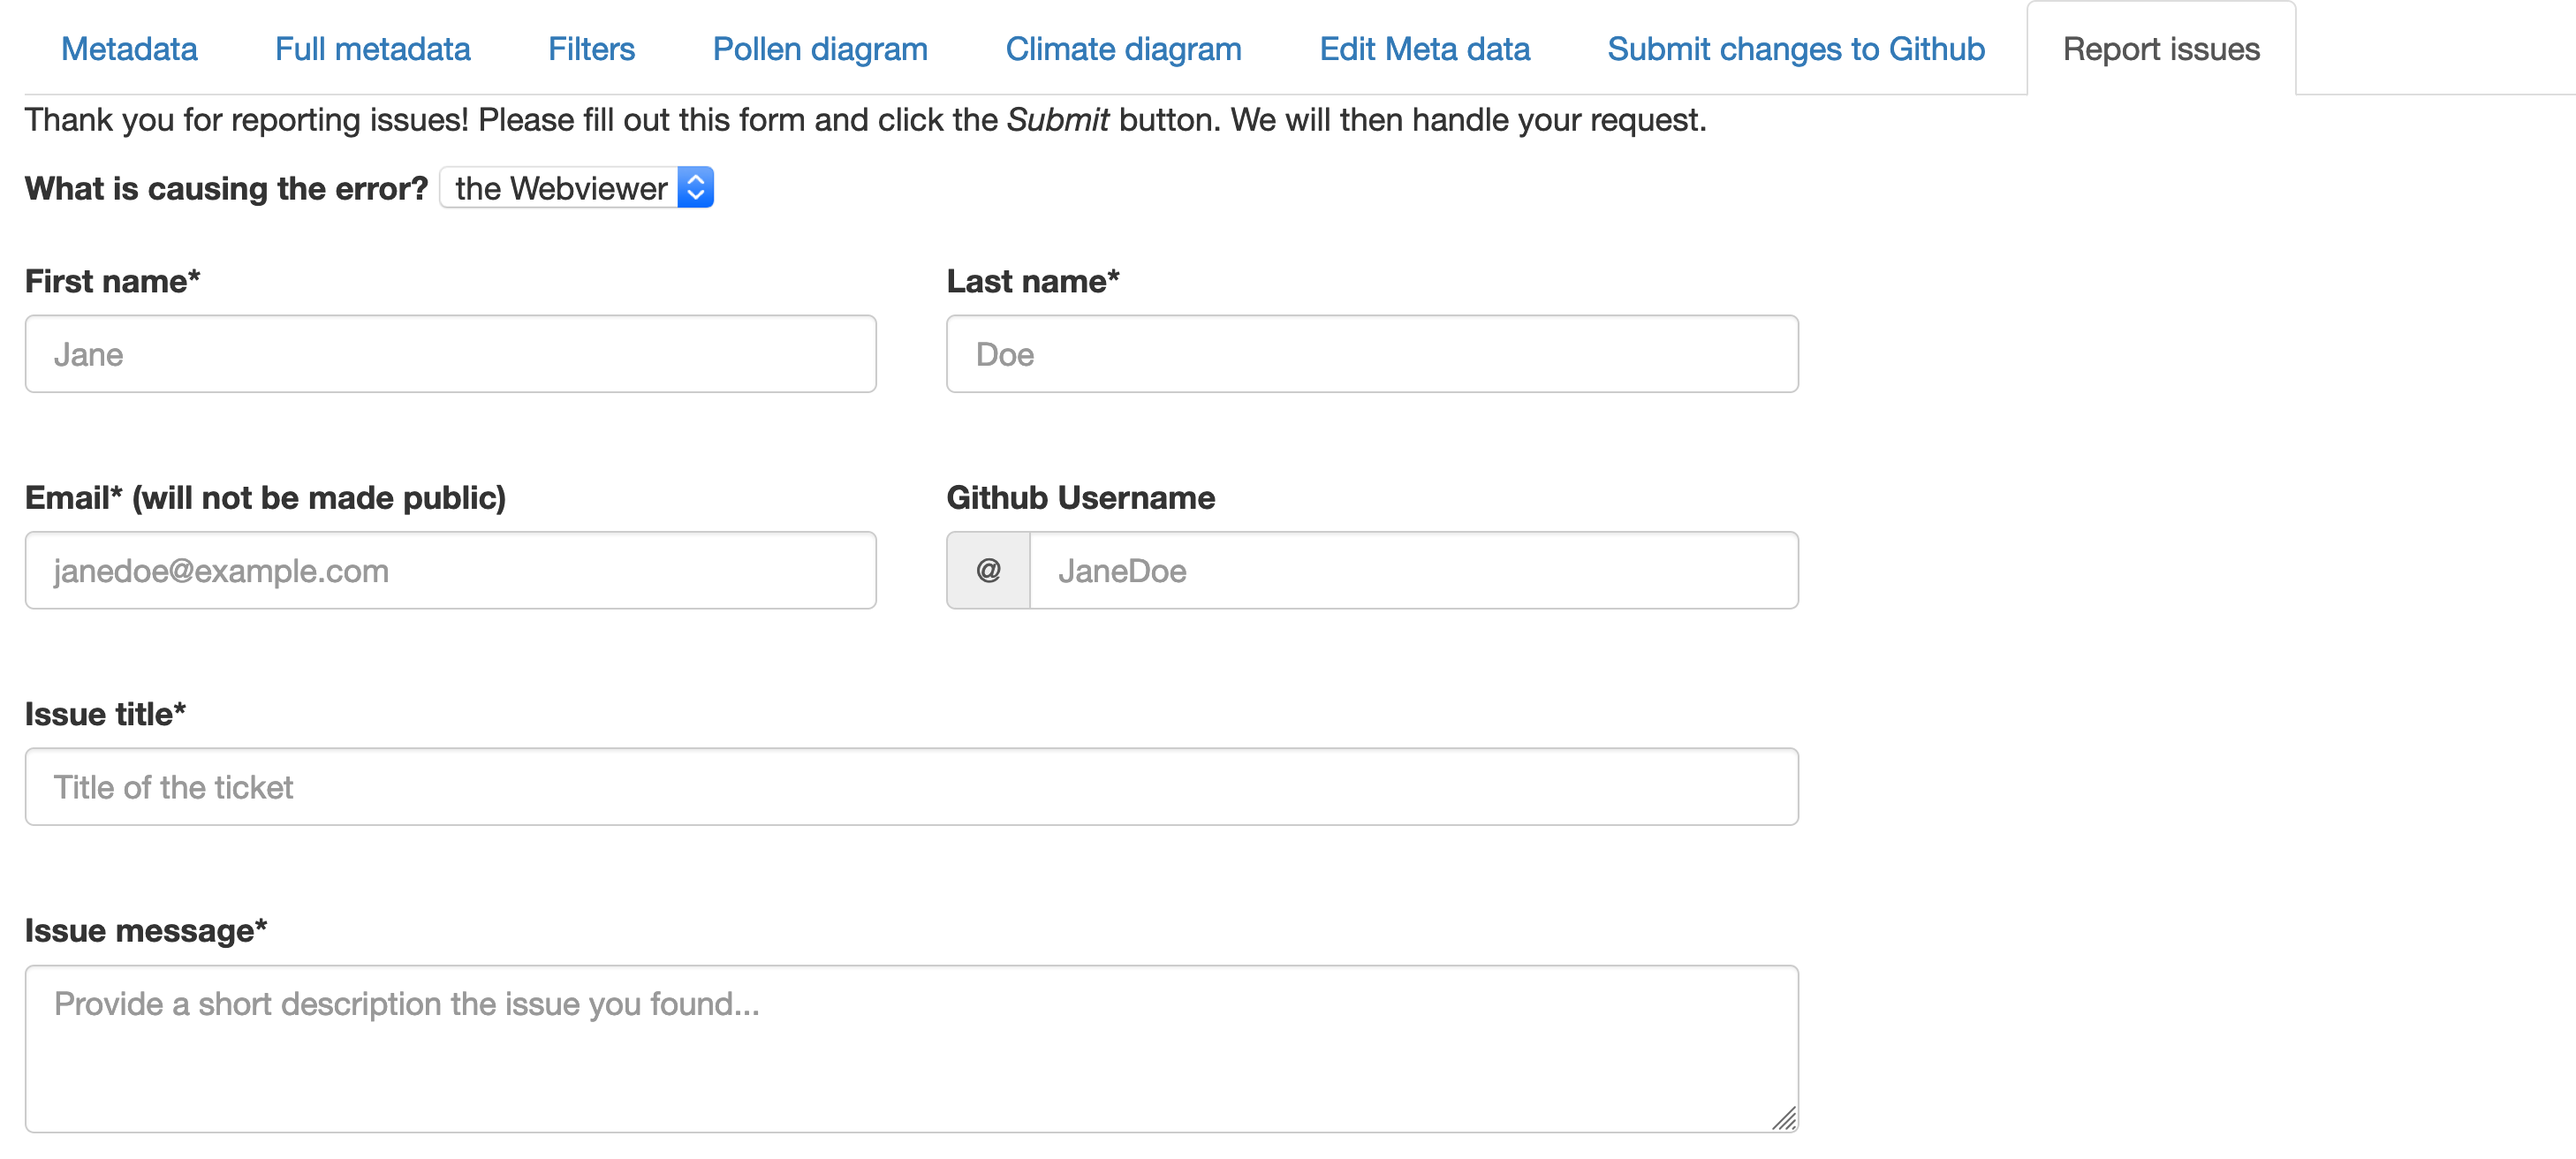
\includegraphics[width=\linewidth]{empd-figures/issue-report.png} \\
		\hline\hline
	\end{longtable}
}

\subsubsection{Implementation details}

The viewer itself is very light-weight and can be flexibly adapted to other database systems (see for example section \ref{sec:polnet-viewer}). As the climate proxies finder \citep{BollietBrockmannMassonDelmotteEtAl2016, Brockmann2016}, the \gls{empd}-viewers main viewing/filtering functionality it is built upon the \textit{dc} \citep{ZhuDevelopers2019}, \textit{crossfilter} \citep{Squarecrossfiltercontributors2019} and \textit{leaflet} \citep{Agafonkin2019} open source JavaScript libraries. We ported the app to the \textit{npm} package manager (\href{https://www.npmjs.com/}{npmjs.com}) which enables a better and more secure monitoring of the app dependencies. This package manager is also used for an automated testing of the viewer on a \gls{ci} service, prior to deployment on the official web page. Due to time constrains, the viewer is not yet fully adapted to mobile devices. 

\subsection{The EMPD2 data repository}\label{sec:empd-data}

The raw data of the EMPD2 is accessible as plain text files in the \textit{EMPD-data} Github repository (see table \ref{tab:empd-links}). The software development framework of Github (see introductory part of section \ref{sec:empd-web-framework}) is adopted such that issues in the data repository can highlight errors in the database, or provide room for the discussion of potential new efforts that should be considered within the community-database. Pull requests into the repository are new data contributions that can be reviewed by the maintainers before being merged into the official database.

This method allows a fully transparent traceback of changes made to the EMPD through version control. The online access to the raw data files through Github also allows the EMPD viewer to interface with different versions of the database (see previous section). 

The EMPD-data repository additionally uses the \gls{ci} services from Travis CI (\href{https://travis-ci.org/}{travis-ci.org}) for automated tests of the meta data in each sample. 


\subsection{The EMPD-admin}\label{sec:empd-admin}

In addition to the standard \gls{ci} services, we developed the \gls{empd}-admin webapp. Inspired by the web management tools of the conda-forge community\footnote{\href{https://conda-forge.org}{conda-forge.org}}, this tool provides an automated handling of data contributions from within Github Pull Requests. It behaves like a standard \gls{ci} service and runs tests on the data contribution, every time changes have been made to the pull request. 

But the main purpose of the EMPD-admin is to provide a web tool for an automated administration of the database, which is helpful for a community-project with changing maintainers. Hence, the \gls{empd}-admin web app acts like a bot that reacts on comments from within a pull request (i.e. a data contribution). Maintainers and contributors can use this functionality and directly contact the bot, for instance, to subset the data, run specific tests on subsets of the data, or automatically fix certain meta data issues, such as wrong countries or missing elevation. 

The bot is also integrated in the \gls{empd}-viewer (see previous section \ref{sec:empd-viewer}). Bug reports or edited data are processed by the \gls{empd}-admin and put online as an issue in the github repository, or it updates the corresponding data contribution.

As such, the administration of the database can be done entirely remotely, without having to install dedicated software on a local computer.

\subsubsection{Implementation details}
The EMPD-admin webapp is hosted for free at Heroku (https://www.heroku.com) at \href{https://empd-admin.herokuapp.com/}{empd-admin.herokuapp.com} with a software package documentation hosted at \href{https://EMPD2.github.io/EMPD-admin}{{EMPD2.github.io/EMPD-admin}}. This, again, allows stability independent on the availability of funding. The package can, also be installed locally and used from the command-line, independent of Github and Heroku, which is sometimes helpful for very large data contributions..

The Python library is based on the tornado web framework\footnote{\href{https://www.tornadoweb.org/en/stable/}{www.tornadoweb.org}}, as well as pandas \citep{McKinney2010}, a tabular data analysis library for Python, and sqlalchemy \citep{Bayer2012}, a Python SQL toolkit.

\subsection{Distribution of the tools}\label{sec:empd-accessibility}

The \gls{empd} is hosted within the \gls{empd}2 Github organization (\href{https://github.com/EMPD2}{github.com/EMPD2}) in the \href{https://github.com/EMPD2/EMPD-data}{{EMPD-data}} repository. The source files of the viewer are accessible in the
\href{https://github.com/EMPD2/EMPD-viewer}{{EMPD-viewer}}, and for the \gls{empd}-admin in the {\href{https://github.com/EMPD2/EMPD-admin}{{EMPD-admin}}} repository (see also table \ref{tab:empd-links}).

The \gls{empd}-data and the \gls{empd}-admin are additionally both available as so-called Docker container image at \url{https://hub.docker.com/u/empd2}. These containers are lightweight, standalone, executable packages of software that include everything needed to run an application: code, runtime, system tools, system libraries and settings. As such, they extend standard software packaging systems by providing an entire operating system that contains the target application. This makes it especially useful for web applications (such as the \gls{empd}-admin) that can, as such, operate in a well-defined and portable environment.

The EMPD-admin can, however, also be installed through the standard python package manager \texttt{pip}.

\section{The POLNET viewer} \label{sec:polnet-viewer}

\begin{figure}
	\centering
	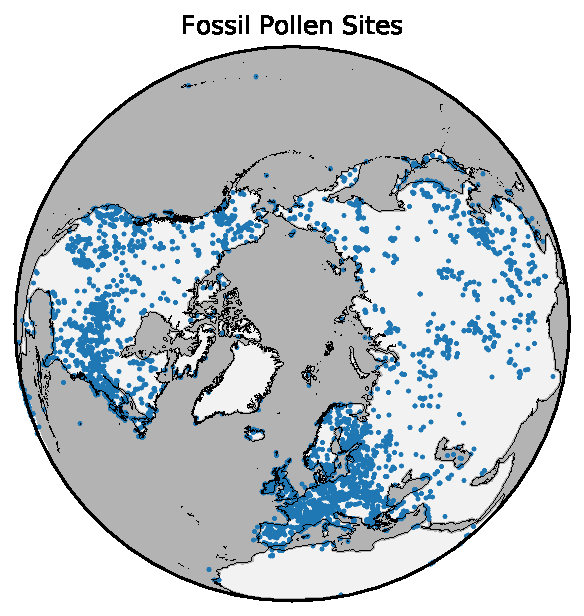
\includegraphics[width=0.45\linewidth]{empd-figures/fossil-sites.pdf}
	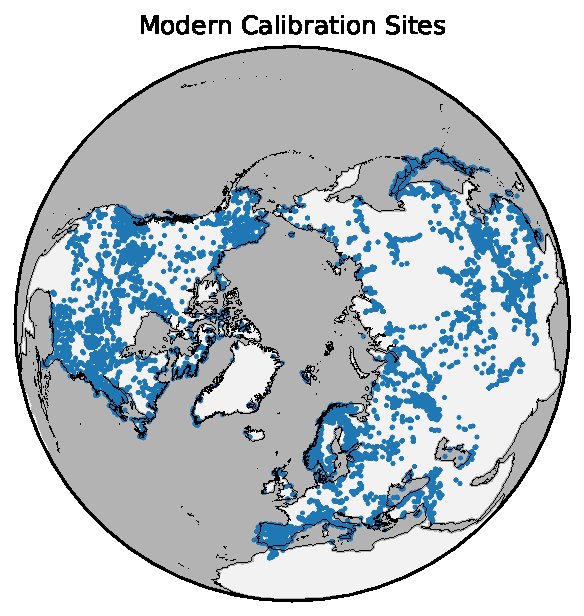
\includegraphics[width=0.45\linewidth]{empd-figures/modern-sites.pdf}
	\caption[Map of sites in the POLNET database]{Maps of (left) fossil and (right) modern pollen sites in the POLNET database.\todo[inline]{obscure grey part in printed version}}
	\label{fig:polnet-sites}
\end{figure}

\begin{figure}[h]
	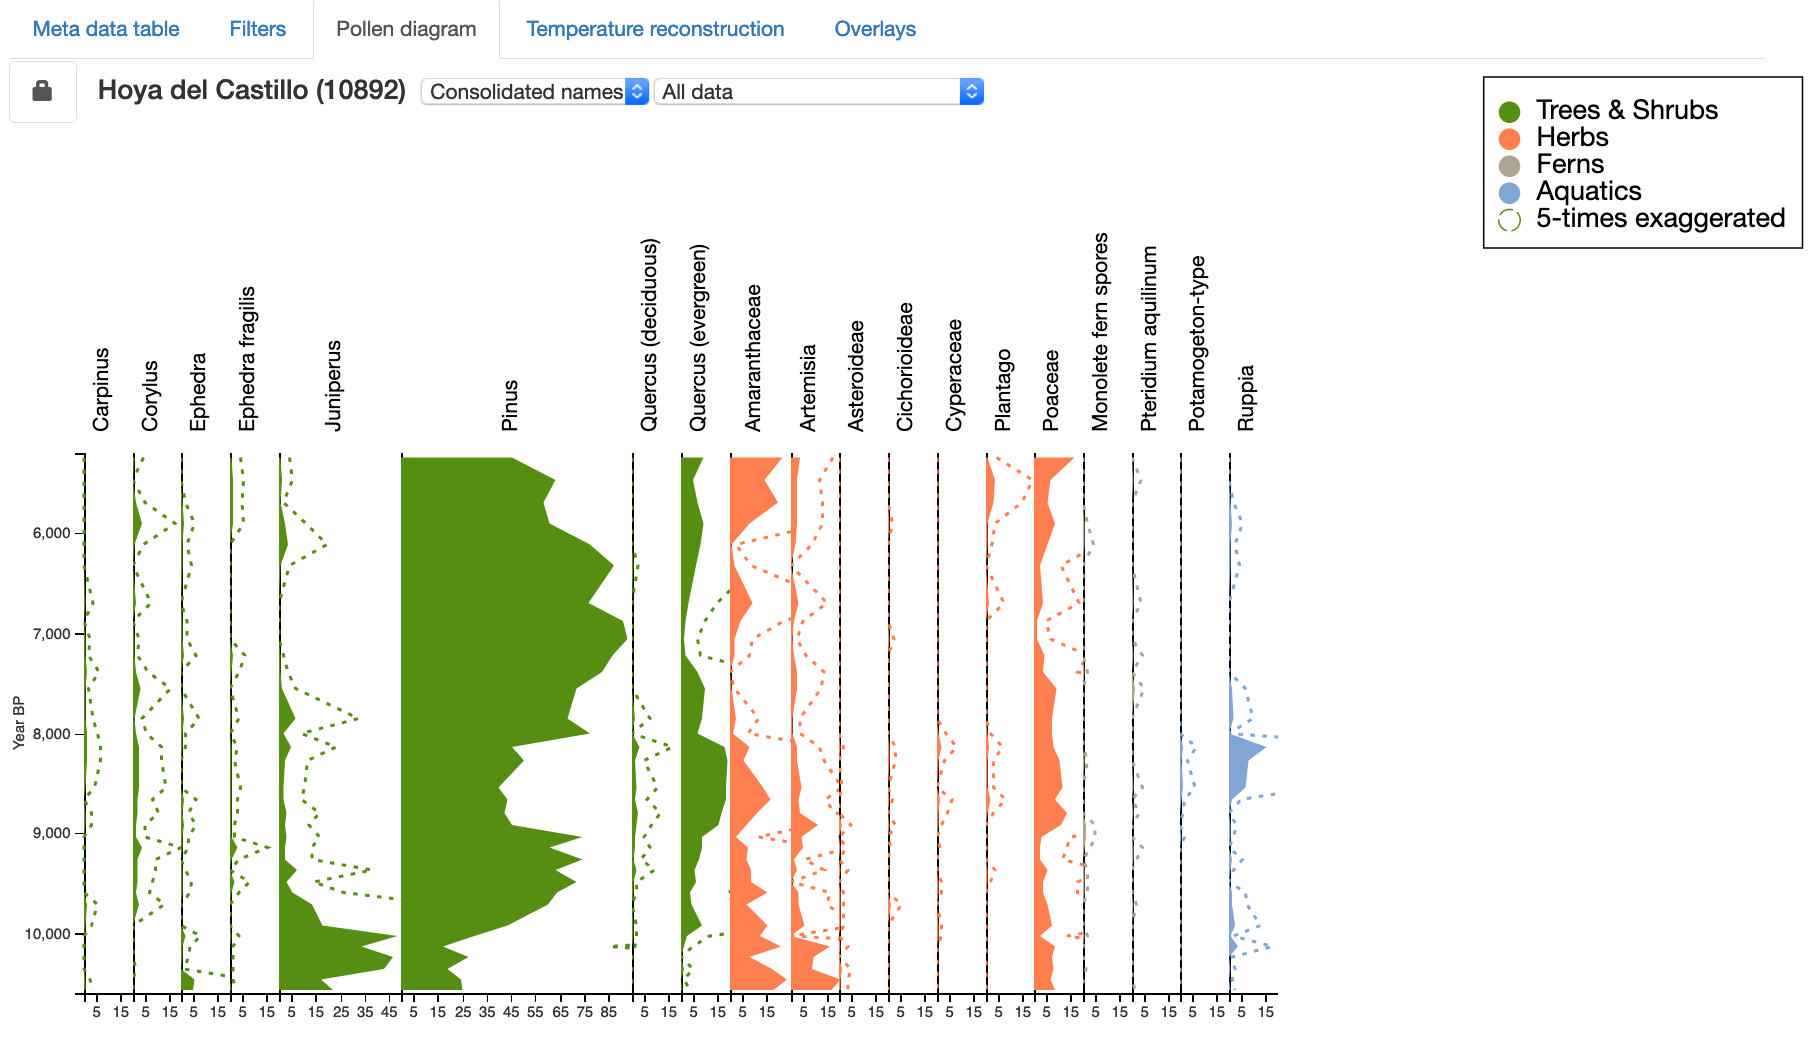
\includegraphics[width=\linewidth]{empd-figures/polnet-diagram.png}
	\caption{Screenshot of an automatically generated pollen diagram in the POLNET database viewer. The left dropdown menu above the pollen diagram allows to select the different naming schemes (here consolidated names that were used for the pollen-climate reconstruction). The right dropdown menu selects either the entire data or specific samples that are then displayed as a bar diagram (see the pollen data in table \ref{tab:empd-viewer-tools}).}
	\label{fig:polnet-pollen-diagram}
\end{figure}

\begin{figure}[h]
	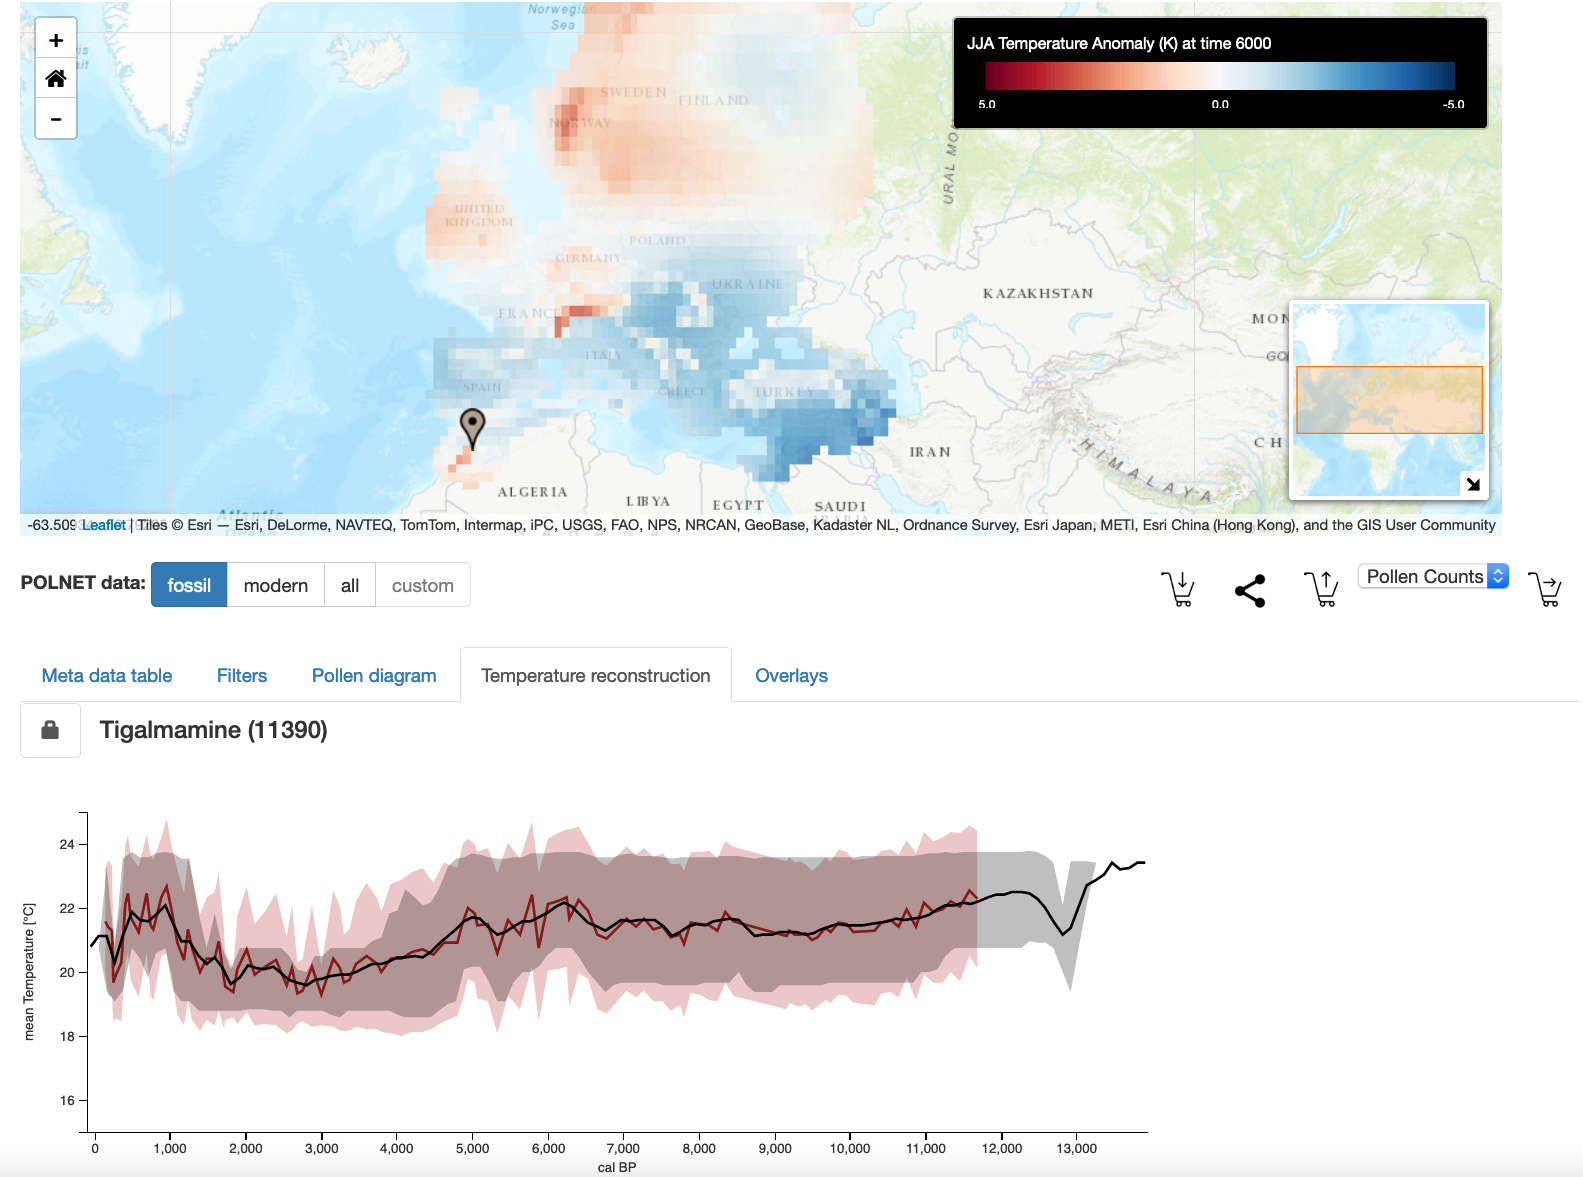
\includegraphics[width=\linewidth]{empd-figures/polnet-climate-plots.png}
	\caption[Climate reconstructions visualized in the POLNET viewer]{Exemplary screenshot how the climate reconstruction is visualized in the POLNET viewer. The map at the top figure shows the gridded temperature reconstruction (here 6k BP after \cite{MauriDavisCollinsEtAl2015}). The lower plot shows the single site-based reconstruction (here Tigalmamine \citep{CheddadiLambGuiotEtAl1998}) for different reconstruction methods.}
	\label{fig:polnet-climate}
\end{figure}

The adaptability of the \gls{empd}-viewer gave the motivation for an application with the POLNET database. This database, currently in development status, is a northern hemispheric, extra-tropical collection of modern and fossil pollen assemblages \citep{DavisKaplan2017, SommerDavisChevalierEtAl2019}. The purpose of this database is to generate the source for large-scale climate reconstruction during the Holocene (past 12'000 years) that can be used for model-data comparisons. It contains about 3'300 fossil pollen sites and about 13'200 modern surface samples (see figure \ref{fig:polnet-sites}) and is at present the largest existing collection of fossil and modern pollen samples. The database will soon be made publicly available through a dedicated web interface, the POLNET viewer. We present it here as a sample application of the EMPD-viewer to demonstrate how this web interface can be extended and applied to other datasets, in order to make them more accessible.

Like its core application, the \gls{empd}-viewer, the POLNET-viewer is a map-based interface with implemented meta data filters. As it is a data exploration and distribution tool only, we did not include the functionalities to edit the meta data or to submit issues. Instead we implemented new features to visualize the essential aspects of this database: fossil pollen data and climate reconstructions.

The fossil pollen data is loaded upon request from the dedicated Github repository. It is afterwards visualized in form of a stratigraphic pollen diagram, with the age of the samples on the vertical y-axis, and the pollen taxa organized as vertically aligned diagram columns (see figure \ref{fig:polnet-pollen-diagram}).

Climate reconstructions are displayed in two different manners: The site-based reconstructions are visualized as line plots in a separate diagram, together with their associated uncertainties. The gridded temperature reconstruction, i.e. the final product of the database (see also chapter \ref{chp:gridding}) is visualized as an overlay on the map of the web application. This results in a combined visualizations of site-based and gridded reconstructions (see figure \ref{fig:polnet-climate}) which enables an intuitive regional analysis of the reconstruction method.

\clearpage

\printbibliography[heading=subbibintoc]

\end{refsection}